\begin{frame}[t,label=problem5]
%\begin{frame}{Algorithms}
    \frametitle{Methods: \textit{De novo} miRNA annotation in \textit{Ciona robusta}}
    \framesubtitle{Re-analysis small RNA-seq data}
    \begin{table}[h!]
        \centering
        \caption{Available SRA small-RNA/miRNA-seq for \textit{C.\ robusta}}\label{tab:experiments}
        \begin{tabular}{ll}
            \toprule
            \textbf{Run} & \textbf{Experiment} \\ \midrule
            SRP002173 & small-RNA for two developmental stages \\ %& Shi W, Hendrix D, Levine M. \\
            SRP079886 & Expression Oral Siphon Regeneration \\ %& Spina EJ, Guzman EB, et al. \\
            SRP116990 & small-RNA transgenic ascidians \\ %& Suntory Foundation \\
            \bottomrule
        \end{tabular}
    \end{table}
    \begin{figure}[h!]
        \centering
        \includegraphics<1>[width=0.8\linewidth]{Figures/solitarytunicate.png} %
        \caption{\textit{Ciona robusta}. Source: Lindsey Leigh, 2017}
    \end{figure}
\end{frame}

\begin{frame}[t]
    \frametitle{Methods: processing patterns $\rightarrow$ miRNAs}
    \framesubtitle{Discovering \textit{de-novo} miRNAs}
    \begin{figure}[h!]
        \centering
        \includegraphics<1>[width=0.5\linewidth]{Figures/workflow2} %
        \includegraphics<2>[width=.65\linewidth]{Figures/workflow3}\label{fig:workflow} %
    \end{figure}
\end{frame}

%\begin{frame}[t]
%    \frametitle{Methods: processing patterns $\rightarrow$ miRNAs}
%    \begin{columns}
%        \begin{column}{0.6\textwidth}
%            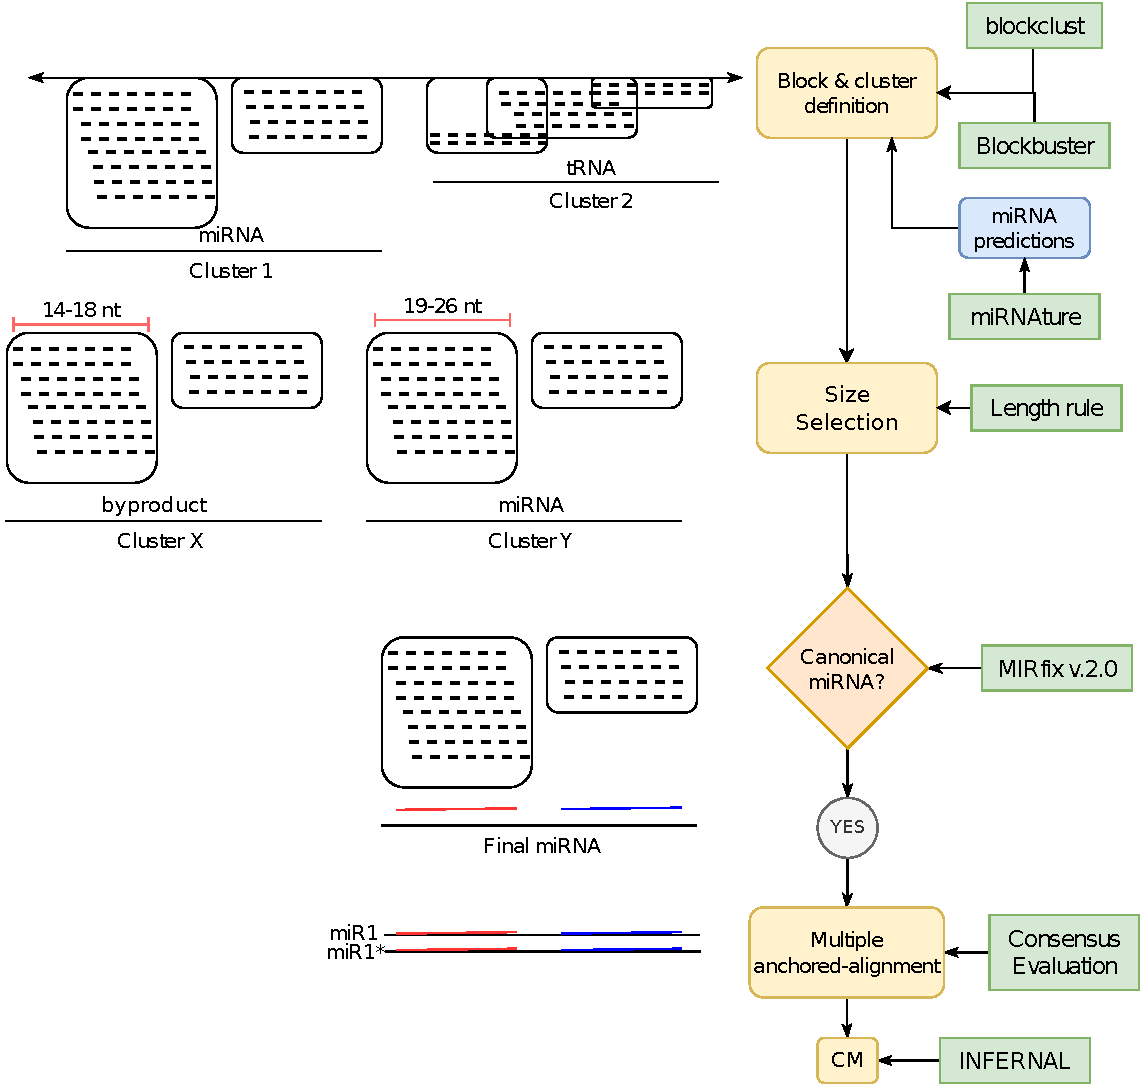
\includegraphics[width=\linewidth]{Figures/workflow3}\label{fig:workflow} %
%        \end{column}
%        \begin{column}{0.4\textwidth}
%            Consensus Evaluation
%            \begin{itemize}
%                \item Base pairs > $18$nt (Cite)
%                \item Number of stems = 1
%                \item Position of 5' \& 3' matures
%            \end{itemize}
%        \end{column}
%    \end{columns}
%\end{frame}
